% Chapter 2

\chapter{Estado da Arte} % Main chapter title
\label{chap:Chapter2} % For referencing the chapter elsewhere, use \ref{chap:Chapter2} 
	Este capítulo apresenta o estado da arte sobre o tema em estudo. Para esse efeito, é descrita a metodologia de investigação adotada para analisar a utilização de modelos de linguagem de grande dimensão no apoio à análise e resolução de incidentes em contextos de operações de \gls{TI}. De seguida, são apresentados os principais artigos obtidos a partir da revisão da literatura, bem como uma discussão dos aspetos comuns e divergentes identificados nesses estudos. Esta análise permite consolidar uma base de conhecimento que serve de suporte à avaliação da viabilidade e à eventual adoção ou desenvolvimento de uma solução para o problema identificado.

%----------------------------------------------------------------------------------------
\section{Metodologia de Investigação}

	Optou-se por utilizar um método de pesquisa com base num estudo sistemático de mapeamento ou \gls{SMS}, a fim de realizar a revisão de literatura. Primeiramente, foi definida uma pergunta de investigação, para estudar soluções já existentes no mercado. De seguida, com base na \gls{RQ} definida e com o suporte da metodologia: \gls{PICOCT}, foram identificados os elementos necessários para estruturar a pesquisa. Com a questão já enquadrada, prosseguiu-se para a definição das palavras-chave e dos limites de inclusão e exclusão. Por fim, para obter os artigos, foram utilizadas bases de dados de artigos científicos reconhecidas, tais como, a \textit{ACM Digital Library} e a \textit{IEEE Xplore}.


	\subsection{Pergunta(s) de Investigação}
		Com base nas dificuldades identificadas pelas equipas \textit{DevOps} e \textit{CorpOps} na análise e resolução de incidentes, surgiu a hipótese de recorrer a ferramentas de \gls{IA}, como técnicas de \gls{PLN}, para apoiar a compreensão e o tratamento destes registos. Desta forma, foi formulada a questão: “\textbf{Como é que as ferramentas de Large Language Models podem melhorar a interpretação e análise de registos de incidentes de TI?}”.
		
	
	\subsection{Metodologia PICOC(T)}
	
		A metodologia \gls{PICOCT} é, geralmente, usada como guia para organizar e clarificar perguntas de investigação, ajudando a estruturar o problema de forma clara. Através desta abordagem, a pergunta é dividida em componentes simples, como a população em estudo, a solução analisada, os resultados esperados e o contexto, tornando mais fácil de perceber o foco da investigação.
		
		Existem várias variantes desta metodologia, como PICO, PCC ou POT, sendo a escolha da variante dependente do tipo de estudo e da área científica. Neste trabalho, a metodologia \gls{PICOCT} foi utilizada para apoiar a formulação da pergunta de investigação e para identificar as palavras-chave usadas na pesquisa bibliográfica.
	
		Com base na pergunta de investigação descrita anteriormente, foi possível realizar a decomposição pelos componentes da metodologia e a obtenção de palavras-chave para cada um desses componentes (Tabela \ref{tab:picoct}).
	
		\begin{table}[H]
			\centering
			\begin{tabular}{|l|p{3cm}|p{3cm}|p{4cm}|}
				\hline
				\textbf{Componente} & \textbf{Descrição} & \textbf{Inclusão/Exclusão} & \textbf{Palavras-Chave} \\
				\hline
				\textbf{P – População} & Registos de incidentes & I — Ferramenta ServiceNow\newline 
				
				E — Estudos sobre gestão de alarmes & "incident management"; "incident analysis"; "incident resolution"; "incident interpretation"; "ticket analysis"; "ticket interpretation"; "ServiceNow" \\
				\hline
				\textbf{I – Intervenção} & Uso de LLMs para análise de incidentes & I — Técnicas conhecidas de LLMs\newline
				
				E — - - - & "Large Language Model"; "LLM"; "Natural Language Processing"; "NLP"; "RAG"; "fine-tuning" \\
				\hline
				\textbf{C – Comparação} & ——— & ——— & ——— \\
				\hline
				\textbf{O – Outcome} & Redução do MTTR, melhoria na priorização e diminuição de erros de analise & I — - - -\newline
				
				E — Estudos não relacionados com incidentes & "incident"; "ticket" \\
				\hline
				\textbf{C – Contexto} & Ambientes DevOps/CorpOps & I — Estudos na área\newline
				
				E — Estudos fora da área & "DevOps"; "CorpOps"; "IT"\\
				\hline
				\textbf{T – Tipo de estudo} & Pesquisa empírica ou com base em estudos & I — - - -\newline
				
				E — Trabalho teórico ou especulativo & Exclude —> "theoretical"; "speculative" \\
				\hline
			\end{tabular}
			\caption[Metodologia PICOCT]{Metodologia PICOCT}
			\label{tab:picoct}
		\end{table}
		
		
	\subsection{Palavras-Chave}
	
		Foi definida uma string de pesquisa (Código \ref{cod:palavrasChave}) com o intuito de orientar a revisão bibliográfica. As palavras-chave utilizadas resultaram da aplicação da metodologia \gls{PICOCT}, garantindo o alinhamento entre a pergunta de investigação e a pesquisa efetuada. Ao longo do processo, a pesquisa assumiu também um caráter exploratório e iterativo, permitindo o ajuste dos termos sempre que necessário, de acordo com os resultados obtidos e com o foco do trabalho. Os termos foram formulados em inglês, de modo a ampliar o número e a relevância dos estudos encontrados.
	
		\begin{lstlisting}[caption={Termos de pesquisa},label={cod:palavrasChave}]
			("incident management" OR "incident analysis" OR "incident resolution" OR "incident interpretation" OR "ticket analysis" OR "ticket interpretation" OR "ServiceNow")
			AND
			("Large Language Model" OR "LLM" OR "Natural Language Processing" OR "NLP" OR "RAG" OR "fine-tuning")
			AND
			("incident" OR "ticket")
			AND
			("DevOps" OR "CorpOps" OR "IT")
			NOT
			("theoretical" OR "speculative")
		\end{lstlisting}
		
		Os termos finais foram posteriormente aplicados com a finalidade de obter os artigos científicos utilizados na investigação.
		
		Os repositórios de pesquisa selecionados, mencionados na Tabela \ref{tab:repositorios}, possibilitaram a consulta de artigos e procedimentos mais fiáveis, relacionados com a área de estudo.
		
		\begin{table}[H]
			\centering
			\begin{tabular}{l l}
				\hline
				\textbf{Repositório} & \textbf{Acesso à plataforma (\textit{URL})} \\
				\hline
				\textit{ACM Digital Library} & \url{https://dl.acm.org/} \\
				\textit{IEEE Xplore} & \url{https://ieeexplore.ieee.org/} \\
				\hline
			\end{tabular}
			\caption[Repositórios de pesquisa]{Repositórios de pesquisa}
			\label{tab:repositorios}
		\end{table}
	
	
	\subsection{Critérios de Inclusão e Exclusão}
		Os critérios de inclusão e exclusão adotados neste trabalho e definidos nas Tabelas \ref{tab:criteriosI} e \ref{tab:criteriosE} são adicionais ao já estipulados na metodologia \gls{PICOCT} e tiveram como principal objetivo delimitar o âmbito da revisão da literatura e garantir a sua relevância para a questão de investigação. São filtros adicionais que não podem fazer parte dos termos de pesquisa mas podem, normalmente, ser configurados nas próprias configurações dos repositórios de pesquisa.
		
		Devido ao elevado número de artigos foi definido no critério \textit{CI1} que, dos procedimentos originários de conferências, apenas seriam considerados trabalhos resultantes da \gls{ICSE}, da \gls{FSE} e a \gls{ASE}.
		
		A \textit{\gls{ICSE}} é uma das principais conferências internacionais, focando-se em inovações e tendências da área. Já a \gls{FSE}, também conhecida como \textit{ESEC/FSE}, destaca-se pelo foco em métodos, ferramentas e técnicas para o desenvolvimento e manutenção de \textit{software}. Por sua vez, a \gls{ASE} centra-se na automação de processos de engenharia de \textit{software}, e em particular nos estudos que envolvem o uso de técnicas de \gls{IA} no apoio a atividades operacionais, como é o caso deste estudo.
		
		\begin{table}[H]
			\centering
			\begin{tabular}{l p{11cm}}
				\hline
				\textbf{Identificador} & \textbf{Critério de Inclusão} \\
				\hline
				\textit{CI1} & Artigos provenientes de conferências reconhecidas e relacionadas com o tema \\
				\hline
			\end{tabular}
			\caption[Critérios de Inclusão]{Critérios de Inclusão}
			\label{tab:criteriosI}
		\end{table}
		
		Com o critério \textit{CE1} procurou-se dar prioridade a trabalhos mais recentes, reduzindo a probabilidade de incluir tecnologias que já não são relevantes.
		
		\begin{table}[H]
			\centering
			\begin{tabular}{l p{11cm}}
				\hline
				\textbf{Identificador} & \textbf{Critério de Exclusão} \\
				\hline
				\textit{CE1} & Publicado antes de janeiro de 2020 \\
				\textit{CE2} & Artigos que não contenham resumo ou \textit{abstract} \\
				\textit{CE3} & Artigos duplicados ou com conteúdos redundantes \\
				\hline
			\end{tabular}
			\caption[Critérios de Exclusão]{Critérios de Exclusão}
			\label{tab:criteriosE}
		\end{table}
		
	
	\subsection{PRISMA}
		Para organizar a revisão de literatura, recorreu-se ao método \gls{PRISMA}, que ajuda a tornar o processo de seleção de estudos \textbf{mais claro e transparente}. Com base nos artigos obtidos nos repositórios de pesquisa, e filtrando esses resultados pelos critérios de inclusão e exclusão, obtivemos os artigos que foram usados como base para esta investigação.
		
		\begin{figure}[H]
			\centering
			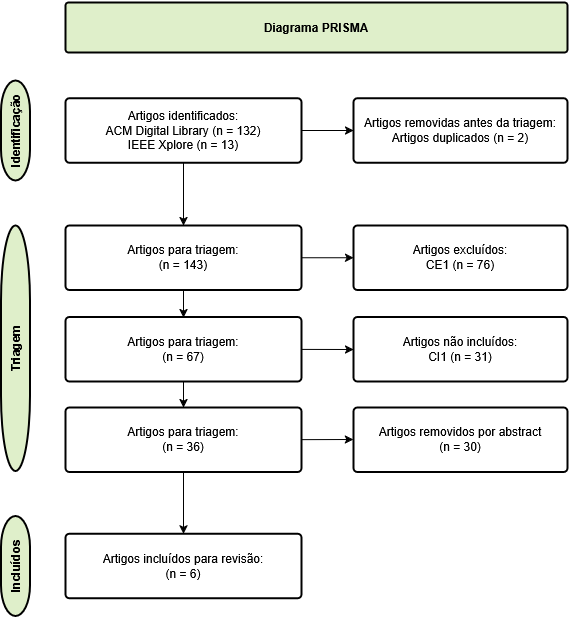
\includegraphics[width=125mm,keepaspectratio]{img/PRISMA}
			\caption[Diagrama \textit{PRISMA}]{Diagrama \textit{PRISMA}}
			\label{fig:prismaDiagram}
		\end{figure}
		
		Como demonstrado na Figura \ref{fig:prismaDiagram}, foram obtidos 145 artigos dos dois repositórios de pesquisa dos quais 2 eram duplicados. Após a identificação inicial, os artigos foram filtrados pelos critérios de exclusão, onde 76 dos mesmos foram descartados por terem sido publicados antes de janeiro de 2020. De seguida, procedeu-se à filtragem pelos critérios de inclusão, que removeu 31 artigos que não se enquadravam nas conferências selecionadas. Por fim, 30 artigos foram excluídos, após leitura do \textit{abstract}, por não se enquadrarem no tema. Sobraram, dessa foram, 6 artigos para analisar na revisão de literatura.
		

\section{Revisão de Literatura}

	Nesta secção, é demonstrada a análise dos resultados obtidos pela metodologia \gls{PRISMA}, abordando os temas por categorias relevantes a esta investigação.
	
	\subsection{Análise de Causa Raiz e Correlação de Incidentes}
		As abordagens atuais para identificar as causas dos incidentes são, ainda, muito reativas e manuais, sendo que toda a investigação da origem do problema depende, quase exclusivamente, da experiência dos \gls{OCEs} e da consulta da documentação técnica e registos das aplicações. Enquanto funcional, para ambientes controlados, estas abordagens tendem a apresentar limitações quando aplicadas a sistemas de grande escala.
		
		Em paralelo, nos ambientes de grande escala, um único problema pode propagar-se por vários serviços e originar múltiplas ocorrências aparentemente independentes, fenómeno já identificado em sistemas reais de gestão de incidentes \autocite{Reference3}. Esta recorrência e repetição de incidentes dificulta a análise realizada pelos \gls{OCEs}, aumento o tempo despendido na procura da causa e do melhor processo de mitigação e conduz, frequentemente, a diagnósticos redundantes ou atrasados. 
		
		Esta recorrência e repetição de incidentes aumenta o tempo investido pelos engenheiros na procura da causa e do melhor processo de mitigação. Assim, torna-se importante identificar correlações entre incidentes que, à primeira vista, pareçam diferentes. Esta ligação entre ocorrências pode ser originária da mesma origem, dos mesmos sintomas ou até de descrições semelhantes. Trabalhos mais recentes mostram que a identificação de relações entre incidentes ou alertas relacionados é fundamental para apoiar atividades como a análise de causa raiz e a mitigação eficiente \autocite{Reference2,Reference1}.
		
		Assim, nos últimos anos, foi evidente o aumento do ênfase na reutilização do histórico de incidentes e na identificação dos padrões recorrentes entre eles. Estudos como \textcite{Reference2} mostraram que a maioria dos incidentes acontecem de forma repetida ao longo do tempo e, muitas vezes, são mitigados utilizado o mesmo procedimento. Este trabalho apresenta o conceito de recomendação automática por meio de \gls{TSG}\textit{s}, demonstrando que a avaliação de incidentes anteriores pode ajudar eficientemente o processo de solução, diminuindo o esforço cognitivo das equipas de operações. De acordo com o mesmo estudo, apenas 27.2\% dos incidentes tinham \gls{TSG}\textit{s} associados, revelando falta de documentação e, principalmente, que em maioria dos incidentes, os engenheiros têm necessidade de investigar a fundo a causa das ocorrências. De notar ainda que, o artigo afirma que, 36.2\% dos incidentes ocorreram pelo menos 2 vezes, podendo levar à reutilização dos métodos de mitigação.
	
		Neste sentido, abordagens baseadas em aprendizagem automática e, mais recentemente, em modelos de linguagem de grande escala têm vindo a ser exploradas para consolidar informação dispersa e apoiar a tomada de decisão durante incidentes complexos \autocite{Reference4,Reference5}, reforçando a importância da correlação de incidentes como etapa central na gestão operacional moderna.
	
	
	\subsection{Sugestões de Mitigação e Uso de Incidentes Anteriores}
		O uso do histórico de incidentes ocorridos é um tema recorrente na literatura, o artigo How to Mitigate the Incident? An Effective Troubleshooting Guide Recommendation Technique for Online Service Systems \autocite{Reference2} foca-se na importância de um \textit{\gls{TSG}} no processo de resolução de incidentes. O estudo analisa a frequência de utilização destes guias e propõe uma ferramenta capaz de recomendar automaticamente o \gls{TSG} mais adequado com base na descrição do incidente. Os resultados demonstram que uma percentagem significativa dos incidentes apresenta padrões repetidos ao longo do tempo, reforçando a relevância da análise histórica. A solução proposta (\textit{D{\small EEP}R{\small MD}}) conseguiu recomendar corretamente o guia mais adequado no Top 1 em cerca de 80\% dos casos, evidenciando o potencial de sistemas de recomendação no apoio à mitigação de incidentes.
		
		\hl{To be continued..}
	
	\subsection{Apoio à Investigação de Incidentes com LLMs}
	
		\hl{To be continued..}
			
	
\section{Conclusão}
	
	- Responder à RQ, com base nos resultados
	- Indicar se vamos então pegar numa solução ou desenvolver uma nova
		Pegar numa até porque todos as soluções utilizaram datasets estáticos
		
	- Apresentação dos resultados
	- Demonstração da relação entre resultados e pergunta de investigação
	- Análise crítica dos  resultados
	- Síntese das principais ilações
	- Identificar as descobertas
	- Registo do que ficou por desenvolver
	- Recomendação de caminhos para futuras investigações
	- Ligar a introdução (objetivos) à conclusão (resultados obtidos)
